\chapter{Introduction}
\label{chap:introduction}
This is a citation: \cite{Vaswani2017}


This is a figure: 

\begin{figure}[ht]
    \centering
    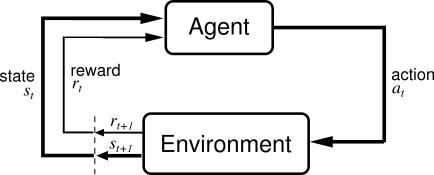
\includegraphics[width=.5\textwidth]{figures/AgentEnviornment.png}
    \caption{I am a caption}
    \label{fig:my_label}
\end{figure}








\section{Contributions}
This work builds upon the researched anomaly detection methods that were established as state of the art over the last years. paper1 and paper2 provide extensive overviews of all SOTA methods,
including the ones mentioned here. The main contributions thus are:
1. Creating a pipeline for anomaly detection experiments and inference, utilizing existing IAD approaches. 
2. Introducing three new categories for the mvtec(LOCO) dataset for anomaly detection experiments.
3. Researching anomaly detection performance on multi perspective datasets.
4. Experiment on the usage of different ensemble methods for IAD, including utilizing neural networks to learn proper ensemble weights.

The above contributions can be used as basis for industrial usage, aswell as a basis for future contributions on ensemble methods in the IAD space. Moreover it gives further insight on the
efficiency of SOTA IAD methods on different kinds of data than the previous synthetic settings.



-- in my work i contribute the following things:
- pipeline to infer new images on different algorithms and compare them
-> pipeline is industry focussed for benefits of the guys where i write my thesis

- research on multi perspective detection

- research of ensemble output learning to enhance individual network performance
-> simple network over 5-6 outputs

- introduction of very new dataset categories in style of mvtec LOCO dataset

